\section{Comparison of {\asas} and {\harps} for period recovery}
\protect\label{section:asasfap}

It seemed appropriate to look in more detail at the {\asas} data which offers \examrevision{a similar sampling cycle,
  based upon ground-based observations,} to that from the {\harps} data discussed in Section \ref{section:harpsper}
above. Of particular importance is the False Alarm Probability for periods recovered from the spectroscopic data as well
as estimating the uncertainty level of all of the calculated periods, particularly those in the photometric data. None
of the three Python routines directly return an FAP and the the {\numrecs} routine always returns an FAP of 1 for the
periods if the periods were found at all. Consequently a Monte Carlo method was devised and implemented to study this
and at the same time help estimate the uncertainty on the period obtained from the {\asas} results.

The {\asas} data has many more observations than the spectroscopic data from {\harps}. The former has 970 and the latter
has 316 (or 260 in the Original Set). If the {\asas} data is binned, then as noted in Section \ref{section:asas}, the
number of observations becomes 924 if binned to the most optimal 18 minutes or 624 if binned to 1 day, more akin to the
binning used in many of the periodicity calculations for the {\harps} data, \examrevision{with a more comparable number
  of observations}.

So, starting from the {\asas} data, binned to 1 day and assuming for the purpose that the 82.6 day period obtained from
the full set as described in Section \ref{section:asas} is correct, various percentage-sized subsets of the data were
randomly selected, recalculating the periods, noting whether a value close to the correct period was recovered as the
strongest peak, within the five strongest peaks, or not at all. If the period was recovered, the RMS error, assessed as
the difference from 82.6 days, was recorded. The sizes of the subsets were taken between 5\% and 95\% in steps of
5\%. For each percentage sized subset, the process was repeated 2,000 times. The results are illustrated in
Fig. \ref{fig:asasprop}.

\examrevision{Four results are shown in Fig. \ref{fig:asasprop}}. In all cases, the X-axis displays the percentage sized
subset of the binned {\asas} data which was used. On the left Y-axis is shown the percentage of recovery (i.e. 100\%
minus the FAP) of the correct period. The blue line shows the percentage recovery of the correct period as the strongest
peak with various percentage sized subsets of the data and the green line shows the percentage recovery of the correct
period as one of the five strongest peaks, not necessarily as the strongest peak. If can be seen that \examrevision{the}
former reaches 100\% recovery at about 70\% and the latter at about 45\%.

On the right Y-axis is shown the RMS error in the period when it is \examrevision{recovered correctly}. The purple line
shows the RMS error in the results corresponding to the case where the correct period is recovered as the strongest peak
and the red line the RMS error in the results corresponding to the case where the correct result is found in one of the
top five peaks. It is noticeable that this reaches less than 0.1 days in both cases, lending weight to the conclusion
that the uncertainty in the 82.6 peak found by {\asas} and {\hst} is of the order of 0.1 days at worst.

Finally, marked in as the dotted vertical black lines are the percentages where various numbers of observations with
various clippings and binnings of the {\harps} data would come. The actual numbers of observations range from 55, or
8.8\% of 624, to 316, or 50.6\% of 624. The intersections with the blue lines would indicate the level of FAP which
would be expected from the most powerful peak in the corresponding periodogram and that with the green lines would
indicate the level of FAP as one of the top five peaks.

\begin{figure}[!htbp]
\begin{center}
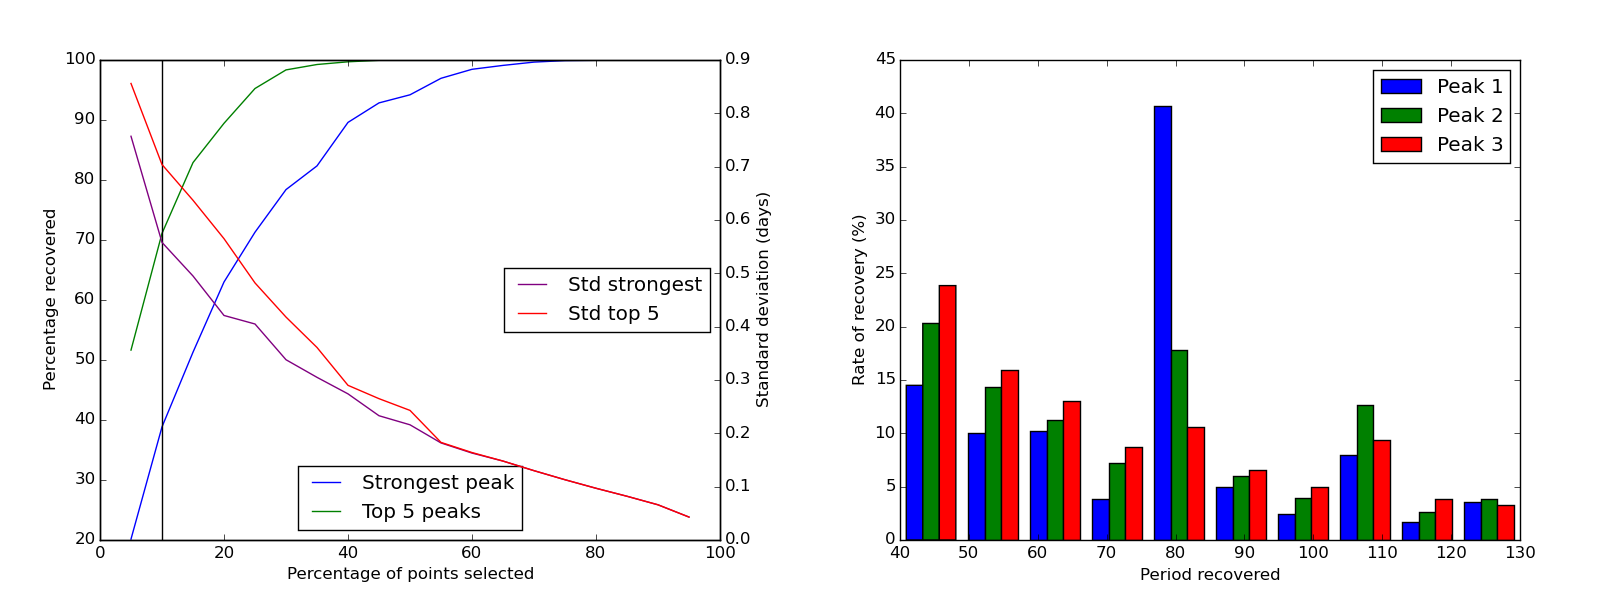
\includegraphics[scale=0.5]{Figures/prop.png} \\
\end{center}   
\caption{In this figure is illustrated the effects of randomly selecting a given proportion of the {\asas} data in terms
  of whether the same period of 82.6 days is recovered and the error in this result. The black vertical dotted lines
  mark in the proportions of data corresponding to the \examrevision{number of observations remaining in the {\harps}
    data after various clippings and binnings have been performed.}}
\protect\label{fig:asasprop}
\end{figure}

\section{Performance summary of spectroscopic measurements}
\protect\label{section:summspec}

\examrevision{Having seen how the performance of the photometric results is affected by the reduction in the number of
  points to those it is useful to compare the variants of spectroscopic measurements against these to assess the
  reliability of each of those. To do this, all of the results of the four measurements studied in this
  {\paperorthesis}, after all variants and combinations of clipping and binning were collated together. In
  Fig. \ref{fig:photcomp1} is shown the comparisons of each of these methods against the ``worst case'' of the subset of
  {\asas} results shown in Fig. \ref{fig:asasprop}. In this figure, the blue bars indicate where each of the
  measurements return 82.6 days to within 0.5\%. (This level of acceptability corresponded approximately to the standard
  deviation of the ``worse case'' of the {\asas} results as shown in Fig. \ref{fig:asasprop}.) It was noticeable that a
  good number of the results returned the likely sub-harmonic of 41.3 days (as given in \citet{benedict93} so the yellow
  bars illustrate this. It is clear that the peak ratio measurement is much the best, whilst the skewness measurement
  never returns the 82.6 day period at all. However all fall well short of the {\asas} results.}

\begin{figure}[!htbp]
\begin{center}
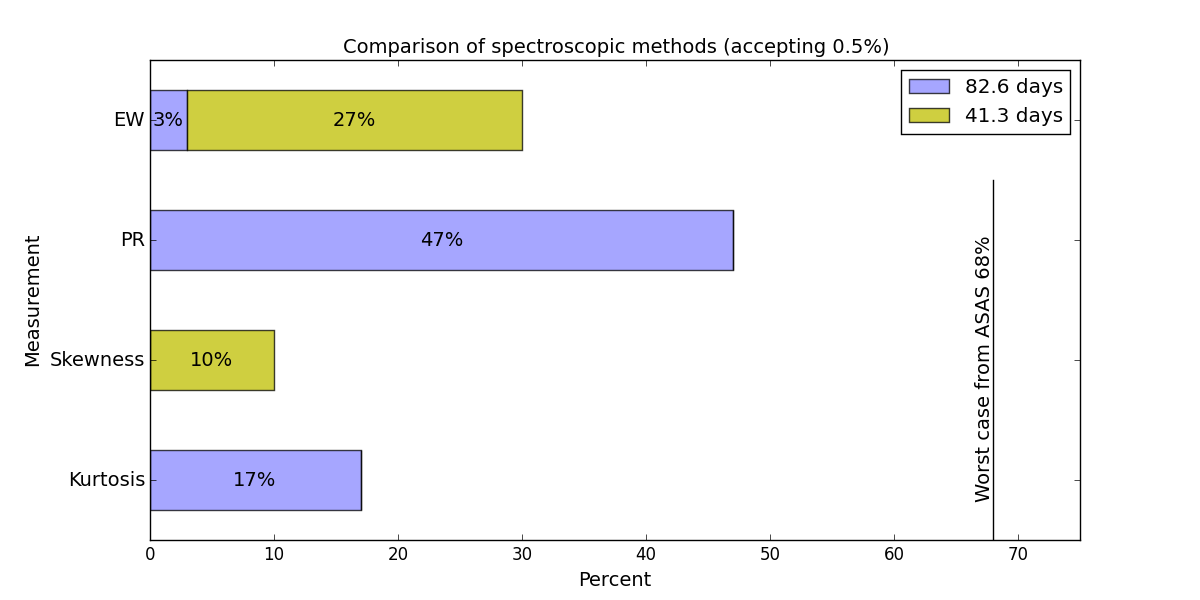
\includegraphics[scale=0.5]{Figures/photcompp5.png} \\
\end{center}
\caption{\examrevision{This figure illustrates the relative performance of each of the 4 spectroscopic methods with the
    Full Set of {\harps} data against the ``worst'' instance of the restriction of the {\asas} points as shown in
    Fig. \ref{fig:asasprop}. In all cases
    it is regarded as ``success'' to recover an 82.6 day period to within 0.5\% as one of the largest five peaks of the
    corresponding periodogram. For each of the four spectroscopic methods considered, all variants of clipping, binning,
    taking residuals and appropriate combinations of those are collated, to give an overall performance for each
    measurement method as a percentage. Shown in blue on the spectroscopic results is the percentage to which 82.6 days
    is recovered. In some cases it was noticed that the 41.3-day sub-harmonic could be recovered and the additional yellow bars denote
    that proportion of the results in which this was noted (where 82.6 days was not also recovered).}}
\protect\label{fig:photcomp1}
\end{figure}

\examrevision{If the threshold of acceptability is relaxed to accept results within 2\%, rather more of the spectroscopic
  results become acceptable, as shown in Fig. \ref{fig:photcomp2}. Both equivalent widths and peak ratio measurements
  return a period within 2\% of 82.6 days half the time, with the former slightly better. It is noticeable that the
  skewness measure considerably improves with this tolerance.}

\begin{figure}[!htbp]
\begin{center}
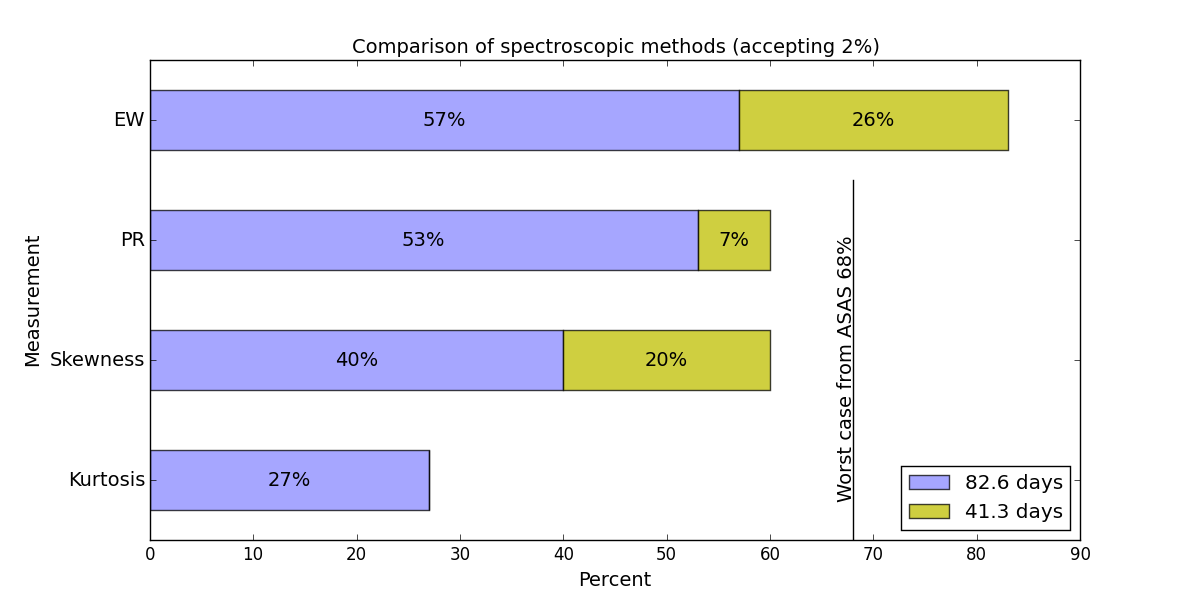
\includegraphics[scale=0.5]{Figures/photcomp2.png} \\
\end{center}
\caption{\examrevision{This figure is Fig. \ref{fig:photcomp1} reworked to illustrate the relative performance of the
    spectroscopic measurements if periods are regarded as valid to within 2\% rather than 0.5\% of 82.6 days (or 41.3 days).}}
\protect\label{fig:photcomp2}
\end{figure}

\examrevision{The performances of these measurements was substantially worse with the Original Set of {\harps} data up
  to 2014. With up to 0.5\% tolerance the equivalent width measure found the 82.6-day period in 5\% of cases as opposed
  to the peak ratio which found it in 38\% of cases, whilst the skewness and kurtosis measurements did not find it at
  all. Improvement was negligible if the tolerance was increased to 2\% or even 5\%.}

\examrevision{It should, of course, be emphasised that this is recovery within the strongest five peaks of the
  periodogram. In only a handful of cases was 82.6 days the strongest peak and those were for the peak ratio measure
  with 1-day binnings.}
